\documentclass{article}
\title{CUDA Parallel Programming\\Homework 2}
\usepackage{graphicx}
\usepackage[UTF8]{ctex}
\CTEXoptions[today=old]
\author{40647007S 朱健愷}

\begin{document}
	\maketitle
	\section{Source codes}
	\subsection{File Layout}
	\begin{itemize}
		\item findMin.cu - Main code containing both CPU and GPU code
		\item Makefile - Script to auto generate executable from code
		\item experiment.sh - Script to auto generate results of matrix addition using different block size
		\item data/Output\textunderscore* - Output result of finding minimum of array using different grid size and block size, the suffix represent the grid size and the block size respectively
		\item notebook/*.png - Plots concluding output result
	\end{itemize}
	
	
	\subsection{Usage}
	Run the experiment.sh script
	
	\begin{verbatim}
	sh experiment.sh
	\end{verbatim}
	
	And it will produce find minimum element in array program's statistical result using different grid size and block size.
	\section{Result}
	\subsection{Experiment environment}
	I ran my code on workstation provided in course, below is the Setup of workstation
	\begin{itemize}
		\item Operating system: Linux version 4.19.172 (root@twcp1)\\(gcc version 6.3.0 20170516 (Debian 6.3.0-18+deb9u1))
		\item CPU: Intel(R) Core(TM) i7-4790 CPU @ 3.60GHz
		\item GPU: Nvidia GTX 1060 6GB
		\item Memory: 32GB 
	\end{itemize}
	\subsection{Performance}
	\subsubsection{Figure}
	\newpage
	\begin{figure}
		\centering
		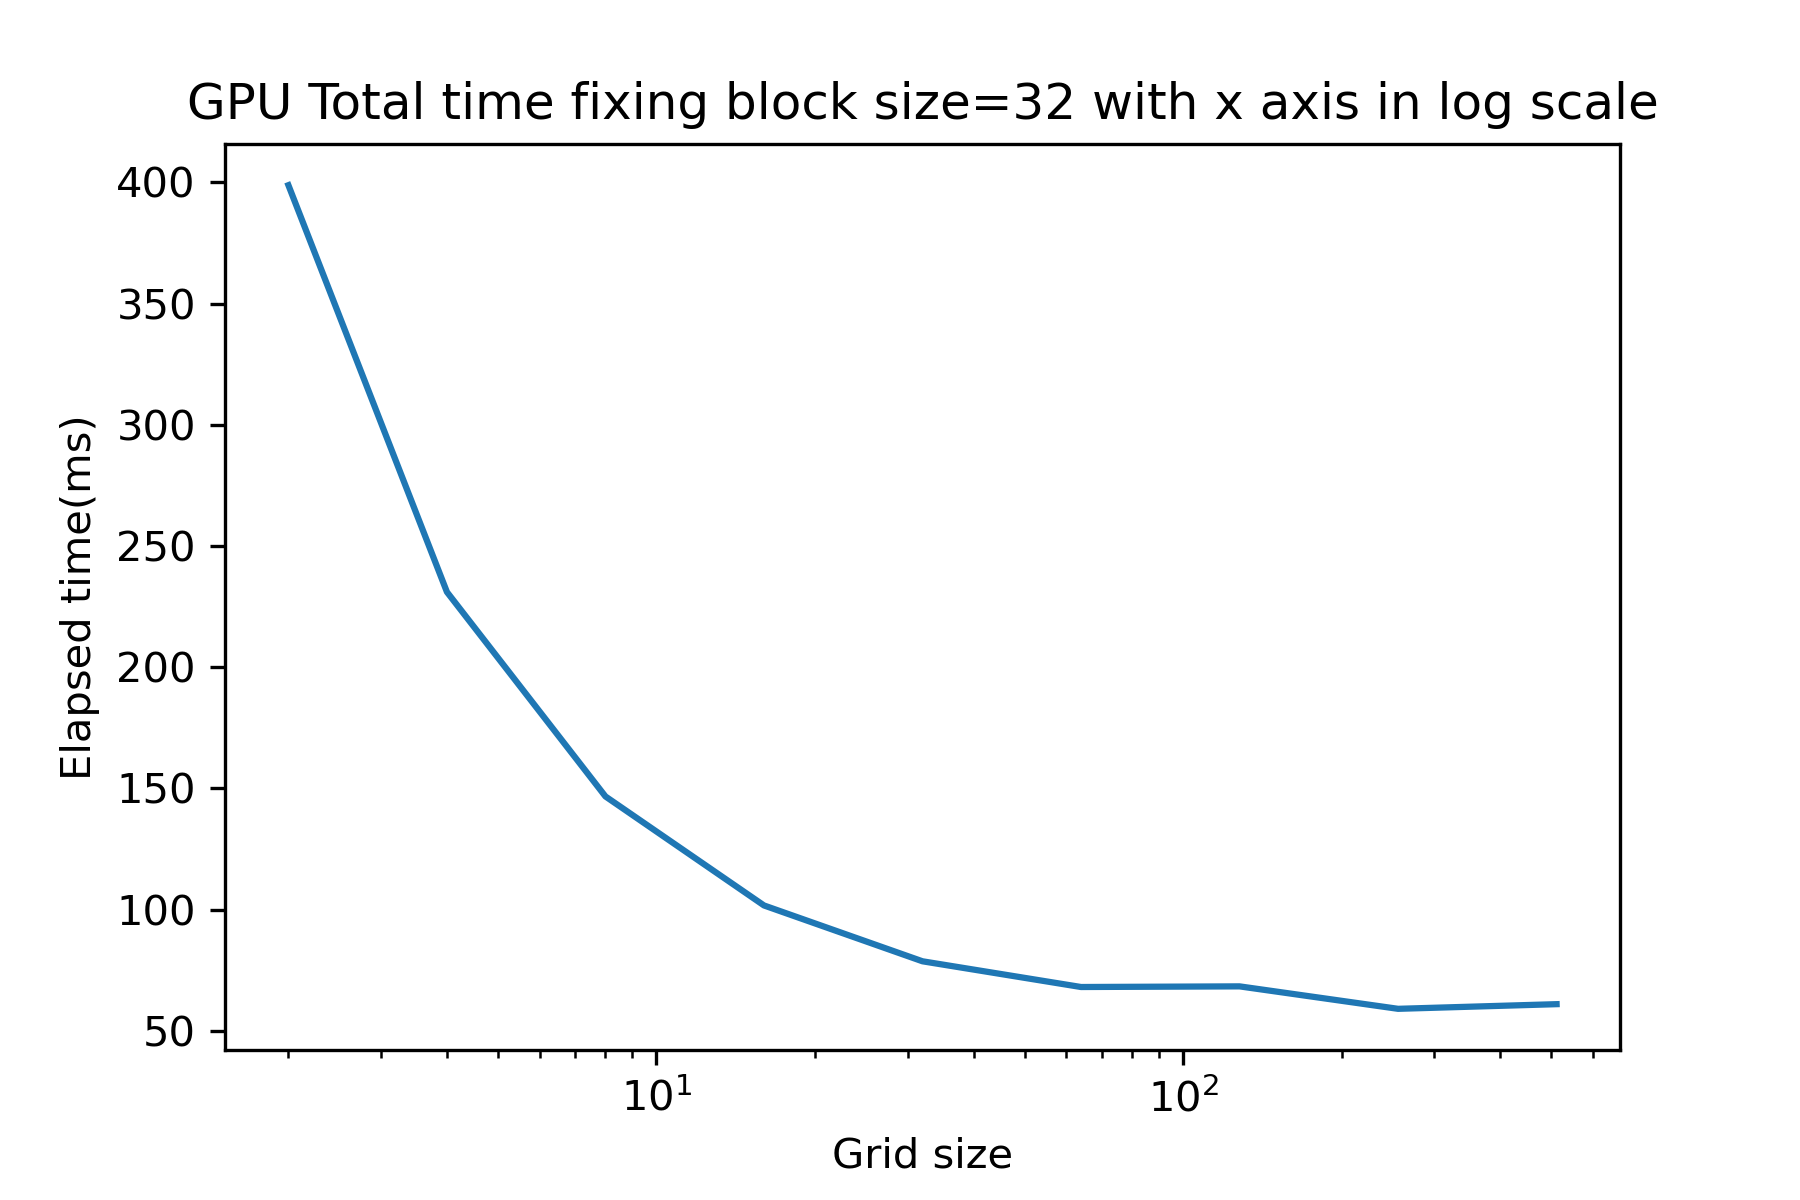
\includegraphics[width=\linewidth]{notebook/gpu_total_time_fixing_block_size}
	\end{figure}
	\begin{figure}[hb!]
		\centering
		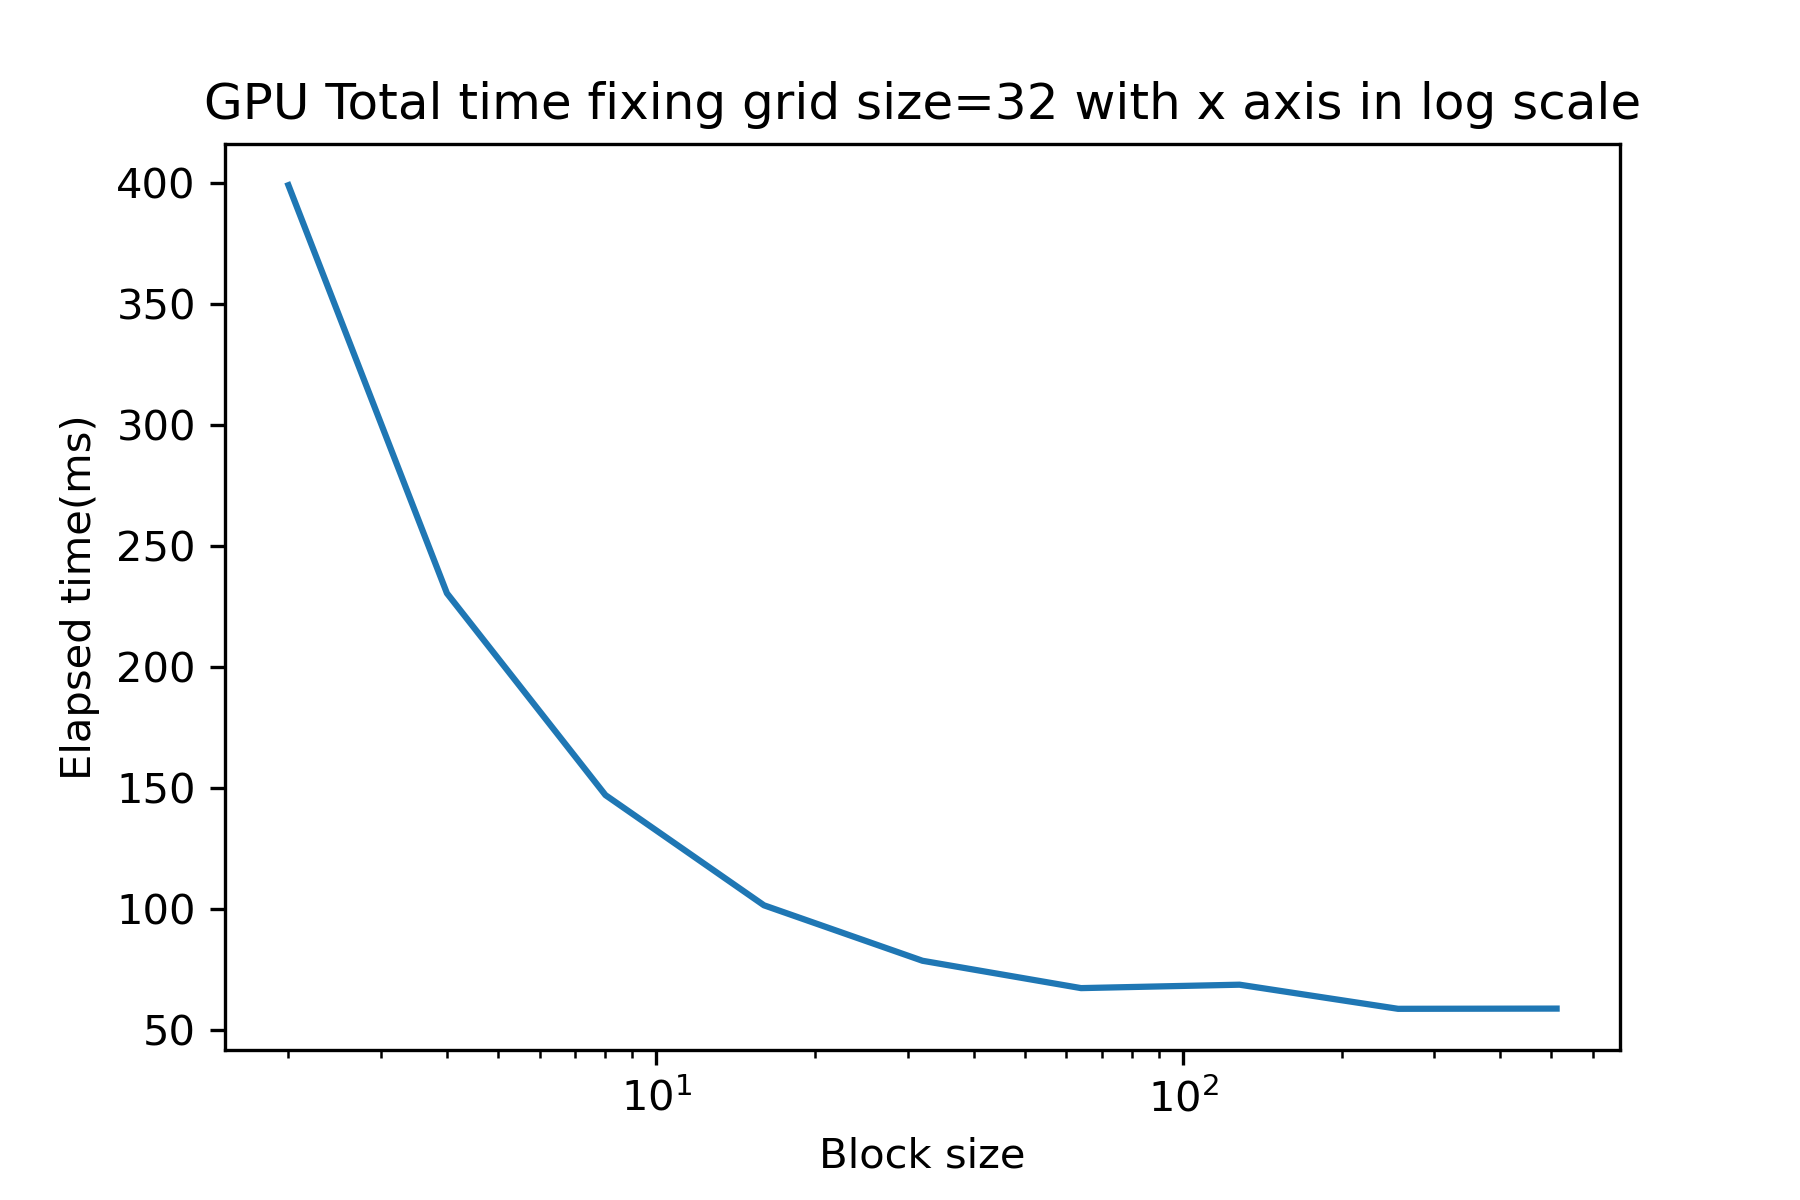
\includegraphics[width=\linewidth]{notebook/gpu_total_time_fixing_grid_size}
	\end{figure}
	\subsubsection{Observation}
	We can observe that the performance of low grid size or low block size setup yields the worse performance in my experiment. This may because of when we do parallel reduction, we usually need many threads in block and many blocks in grid in order to collect minimum element in specific range of array, and then gather the result using CPU. So the block size and grid size do affect the performance a lot.
	
	Same as the observation I observed in the previous assignment, the performance increase until grid size or block size increase to some extent. 
	
	\section{Discussion}
	Parallel reduction do requires more grid size and block size to speed up because it collects each thread's result into blocks using GPU, and collects each block's result as the answer using CPU. 
	
	I've wondered that why not using GPU to collect the final answer from each block, but after having discussion with my classmates I realised that I've mistaken that there is no shared memory between block, so I can't do that. 
	
\end{document}